\chapter{Где учатся и кем работают изобретатели языков программирования}
\label{ch:programming languages}

В статье исследуются свойства языков программирования на основе базы знаний международного проекта Викиданные. С помощью SPARQL-запросов, вычисляемых на объектах типа "язык программирования" в Викиданных, решен ряд задач. Получены перечени всех языков программирования под пермиссивными лицензиями и языков с закрытыми лицензиями и рассчитано их процентное соотношение. Построена пузырьковая диаграмма по количеству форматов файлов исходного кода. Получены карты, отображающие месторасположение учебных заведений и компаний, в которых учились или работали люди, связанные с созданием языков программирования. Построена пузырьковая диаграмма, отображающая профессии людей, причастных к созданию и разработке языков программирования. Получен список всех объектно-ориентированных языков программирования и сделан вывод об исчерпывающей полноте Викиданных относительно них. Проведено сравнение и анализ результатов SPARQL-запросов 2017 года и 2020 года, отмечены основные изменения. 

\section{Количество форматов файлов исходного кода}

В зависимости от языка программирования, файлы с исходным кодом программ могут иметь разные расширения. Построим пузырьковую диаграмму по количеству допустимых форматов файлов исходного кода и сравним с аналогичной диаграммой, построенноый в 2017 году.

%\begin{marginfigure}
%{
%\setlength{\fboxsep}{0pt}%
%\setlength{\fboxrule}{1pt}%
%\fcolorbox{white}{white}{\includegraphics[width=\linewidth]{./chapter/programming_language/%File_extensions_quantity_of_source_code_2017.png}}%
%}
%  \caption{Пузырьковая диаграмма по количеству форматов файлов исходного кода на 2017 год.}%
%  \label{fig:source_files_format_2017}%
%\end{marginfigure}
%
%\begin{marginfigure}
%{
%\setlength{\fboxsep}{0pt}%
%\setlength{\fboxrule}{1pt}%
%\fcolorbox{white}{white}{\includegraphics[width=\linewidth]{./chapter/programming_language/%File_extensions_quantity_of_source_code_2020.png}}%
%}
%  \caption{Пузырьковая диаграмма по количеству форматов файлов исходного кода на 2020 год.}%
%  \label{fig:source_files_format_2020}%
%\end{marginfigure}

На рисунке рис. ~\ref{fig:source_files_format_2017} видно, что на 2017 год самыми исторически богатыми на форматы и расширения файлов являлись такие языки программирования, как: C++ (10 форматов), Geometric Description Language (8), Racket (7). Причем стоит заметить, что соотношение один язык программирования - один формат файлов исходного кода не является верниы. Например, файлы с программой на языке Racket могут иметь расширения rkt, rktl, rktd, scrbl, plt, ss или scm.

\begin{figure}[h]
\centering
	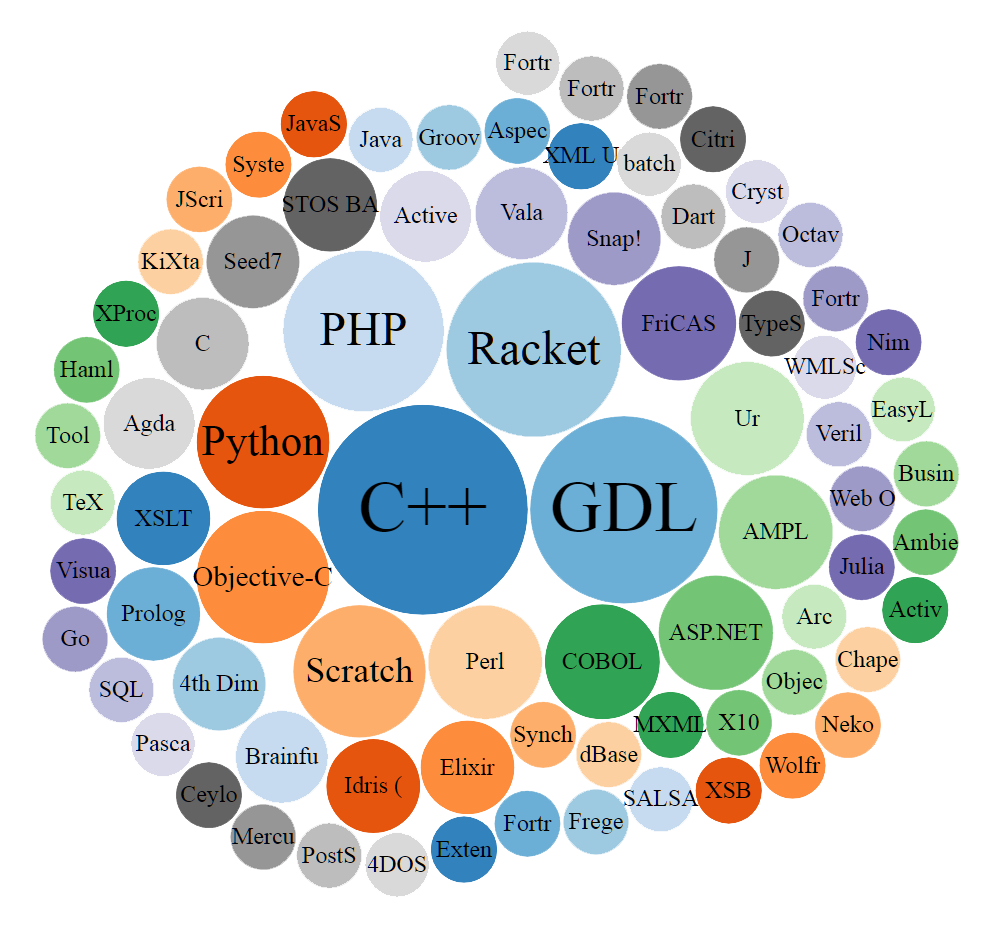
\includegraphics[width=0.7\textwidth]{./chapter/programming_language/File_extensions_quantity_of_source_code_2017.png}
	\caption{Пузырьковая диаграмма по количеству форматов файлов исходного кода на 2017 год.}
	\label{fig:source_files_format_2017}
\end{figure}

К 2020 году (рис. ~\ref{fig:source_files_format_2020}) C++ и Geometric Description Language (GDL) остались на лидирующем месте (10 и 8 форматов-расширений). За три года подтянулись и вошли в первую восьмёрку также такие языки, как Raku (9 форматов), REXX и Scratch (по 6 форматов), Java и Wolfram Language (по 5 форматов).

\begin{figure}[h]
\centering
	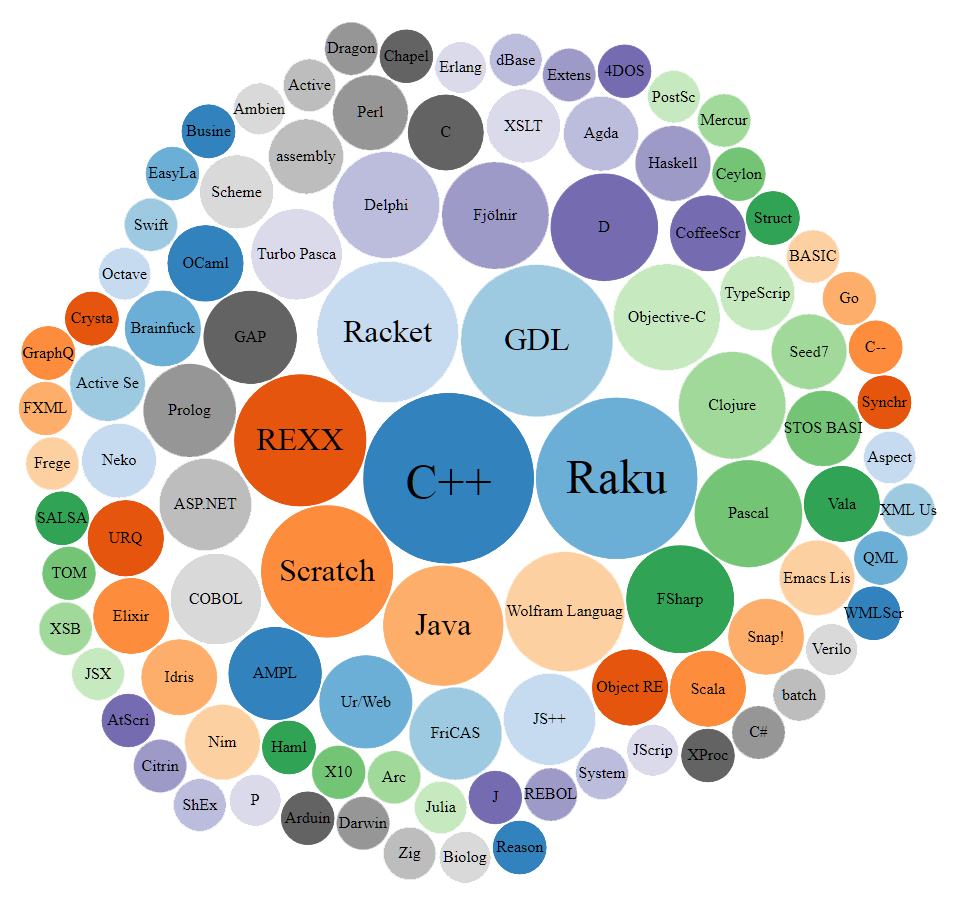
\includegraphics[width=0.7\textwidth]{./chapter/programming_language/File_extensions_quantity_of_source_code_2020.png}
	\caption{Пузырьковая диаграмма по количеству форматов файлов исходного кода на 2020 год.}
	\label{fig:source_files_format_2020}
\end{figure}

Из этого можно сделать вывод, что развитие языков программирвоание продолжается непрерывно, постоянно возникают новые форматы файлов исходного кода, но лидеры в этой области не спешат сдавать свои позиции.